\documentclass[12pt,a4paper,twoside]{article}
\usepackage{geometry}
\geometry{a4paper}

\usepackage{pgfplots} %wykresy
\usepackage[utf8]{inputenc}
\usepackage[OT1]{fontenc}
\usepackage{polski}
\usepackage{graphicx} %wstawianie obrazków
\usepackage{epstopdf} %wstawianie obrazków w formacie .eps
\usepackage{setspace}
\usepackage{fancyhdr} %nagłówki i stopki na każdej stronie
\usepackage{amsmath}
\usepackage{amssymb}
\usepackage{enumitem}
\usepackage{microtype}
\usepackage{url}
\usepackage{floatrow} %domyślnie wyśrodkowuj ryciny

\pgfplotsset{compat=1.5} %wersja biblioteki do wykresów; usuwa problemy
\newcounter{attcounter} %licznik załączników

\begin{document}
\newgeometry{margin=3cm}
\onehalfspacing
\newcommand{\myparagraph}[1]{\paragraph{#1}\mbox{}\\}

\begin{titlepage}
    \begin{center}
    {\LARGE Uniwersytet im. Adama Mickiewicza w Poznaniu \\
    Wydział Matematyki i Informatyki }
    \line(1,0){350}

    \vspace{1cm}
    
\includegraphics[width=2cm]{logo-uam/logo-uam.png}
    \vspace{1cm}

    \vspace{1cm}
    {\Huge Ataki na kryptograficzne \\ funkcje skrótu} \\[0.5cm]
    {\Large Marcin Kurczewski}
    \end{center}

    \vspace{3cm}
    \hspace{8cm}\parbox[l]{6cm}{\Large Praca magisterska \\
    napisana pod kierunkiem \\
    dr Michała Rena}

    \begin{center}
    \vspace{4cm}
    Poznań, maj 2013
    \end{center}
\end{titlepage}


\newpage
\thispagestyle{empty}
\begin{center}
    OŚWIADCZENIE
\end{center}

Ja, niżej podpisany Marcin Kurczewski, student Wydziału Matematyki i
Informatyki Uniwersytetu im. Adama Mickiewicza oświadczam, że przedkładaną
pracę dyplomową pt.: "Ataki na kryptograficzne funkcje skrótu" napisałem
samodzielnie. Oznacza to, że przy pisaniu pracy, poza niezbędnymi
konsultacjami, nie korzystałem z pomocy innych osób, a w szczególności nie
zlecałem opracowania rozprawy lub jej części innym osobom, ani nie odpisywałem
tej rozprawy lub jej części od innych osób.

Oświadczam również, że egzemplarz pracy dyplomowej w formie wydruku
komputerowego jest zgodny z egzemplarzem pracy dyplomowej w formie
elektronicznej.

Jednocześnie przyjmuję do wiadomości, że gdyby powyższe oświadczenie okazało
się nieprawdziwe, decyzja o wydaniu mi dyplomu zostanie cofnięta.


\newpage
\setcounter{tocdepth}{3}
\tableofcontents

\newpage
\pagestyle{fancy}
\fancyhead[L]{\fontsize{10}{0}\selectfont
    Ataki na kryptograficzne funkcje skrótu}
\fancyhead[R]{\fontsize{10}{0}\selectfont
    Marcin Kurczewski}


\section{Wstęp}
Celem tej pracy jest przedstawienie współczesnych metod łamania
kryptograficznych funkcji skrótu, zarówno od strony praktycznej, jak i
teoretycznej. Jako główny temat technologiczny zostały wybrane funkcje
\texttt{MD5} oraz \texttt{SHA-1}.

Praca złożona jest z trzech części. Pierwsza stanowi wprowadzenie do tematyki
kryptograficznych funkcji skrótu, opisując krótko ich rys historyczny,
zgłębiając szczegółowo budowę i przedstawiając ich zastosowania.

Druga część opisuje szereg uniwersalnych technik, które można zastosować do
atakowania większości współczesnych kryptograficznych funkcji skrótu w sposób
niezależny od ich struktury. W części tej są także przedstawione podstawowe
metody obrony przed tego typu atakami.

Część trzecia prezentuje od strony technicznej wybrane wysoce wyspecjalizowane
ataki teoretyczne, jakie powstały na przestrzeni ostatnich lat, pokazując luki
w kryptograficznych funkcjach skrótu.

\newpage



\section{Wprowadzenie do tematyki}

\subsection{Terminologia użyta w pracy}

Zgodnie z terminologią stosowaną w kryptologii, w pracy konsekwentnie
wykorzystywane będą następujące pojęcia:

\begin{itemize}
\item \textbf{funkcja haszująca} -- alternatywne określenie na \emph{funkcję
skrótu},
\item \textbf{bezpieczna funkcja haszująca} -- alternatywne określenie na
\emph{kryptograficzną funkcję skrótu},
\item \textbf{zwykła funkcja haszująca} -- funkcja skrótu, która może, ale nie
musi być \emph{kryptograficzną funkcją skrótu},
\item \textbf{wiadomość} -- wartość wejściowa dla \emph{funkcji skrótu},
\item \textbf{skrót} -- wartość wyjściowa z \emph{funkcji skrótu},
\item \textbf{hasz} -- alternatywne określenie na wartość wyjściową
\emph{funkcji skrótu},
\item \textbf{kolizja} -- sytuacja, w której skróty dwóch wiadomości są takie
same, tj.
\[
    \begin{aligned}
    m &\neq m' \\
    H(m) &= H(m')
    \end{aligned}
\]
\item \textbf{\textit{random oracle}} -- teoretyczna funkcja działająca na
zasadzie "czarnej skrzynki" (o której działaniu nie potrafimy nic powiedzieć),
przypisująca wejściom w losowy, ale deterministyczny odpowiednie wyjścia z
jednostajnym rozkładem prawdopodobieństwa.
\item \textbf{zadanie praktycznie niewykonalne} -- algorytm, który realizuje
dane zadanie, nie istnieje, albo jego koszt obliczeniowy lub pamięciowy jest
tak wielki, że nie można go wykonać przy pomocy znanych obecnie technologii.
\end{itemize}

Dodatkowo, od części~\ref{sec:hash_construction} do końca pracy przez pojęcie
funkcji haszujących będziemy rozumieć wyłącznie kryptograficzne funkcje
haszujące, gdyż tylko na takich funkcjach w tych częściach będziemy się
skupiać.
\pagebreak



\subsection{Definicja zwykłej oraz kryptograficznej funkcji skrótu}

Funkcja skrótu jest to funkcja, której dziedziną są ciągi bitów dowolnej
długości, a przeciwdziedziną -- ciągi bitów o ograniczonej długości. Rzutowanie
to odbywa się w sposób jednoznaczny, tj. każdemu wejściu funkcja skrótu
przyporządkowuje dokładnie jedno wyjście; formalnie zatem jest to surjekcja:

$$ f \colon X \to Y $$
$$ |Y| \leq n, n \in \mathbb{N} $$
$$ \forall_{y \in Y} \; \exists_{x \in X} \; f(x)=y $$

\begin{figure}[htb!]
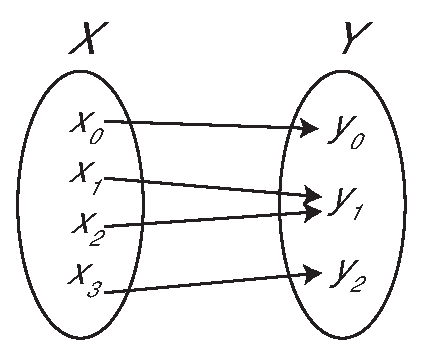
\includegraphics[width=6cm]{img/surjection.eps}
\caption{Każdemu wejściu przyporządkowywane jest dokładnie jedno wyjście}
\label{fig:surjection}
\end{figure}

Kryptograficzna funkcja skrótu to taka funkcja skrótu, która może być
wykorzystywana w zastosowaniach kryptograficznych, a więc wymagających
wysokiego poziomu bezpieczeństwa. Przykłady takich zastosowań można znaleźć w
sekcji~\ref{sec:secure_hash_usages}. Dokładne cechy, jakie powinna spełniać
funkcja skrótu, aby była kryptograficzna, omówione zostały w sekcji
~\ref{sec:secure_hash_attributes}. Ponadto wszystkie funkcje skrótu,
niezależnie od swojego zastosowania w celach kryptograficznych, powinny
spełniać własności opisane w sekcji~\ref{sec:common_hash_attributes}.



\subsubsection{Cechy zwykłych funkcji haszujących}
\label{sec:common_hash_attributes}
Niezależnie od swojego zastosowania, każda funkcja haszująca musi spełniać
pewne warunki, które zostały poniżej opisane.

\myparagraph{Determinizm}
Funkcje haszujące powinny być deterministyczne w takim sensie, że ich wyniki
zależą wyłącznie od danych wejściowych, a nie żadnych czynników losowych.
Innymi słowy, haszowanie wiadomości $m$ powinno dawać taki sam skrót
niezależnie od okoliczności. Stąd wynika, że funkcje skrótu nie powinny się
nigdy odwoływać do generatorów liczb pseudolosowych, metadanych o wiadomości
(typu jej lokalizacja w pamięci komputera) itp., a jedynie do samej wiadomości.

\myparagraph{Jednostajność}
Niech $H : A \to B$ będzie funkcją haszującą. Funkcje haszujące powinny mapować
wartości ze zbioru wejściowego $A$ na wartości ze zbioru wyjściowego $B$ w taki
sposób, by:
\[
    \forall_{a \in A} \; \Pr(H(a) = b) \to \frac{1}{|B|}
\]
Innymi słowy dobra funkcja haszująca mapuje konkretną wartość $a$ w konkretną
wartość $b$ z prawdopodobieństwem jak najbliższym prawdopodobieństwu losowego
wybrania tego elementu ze zbioru $B$, lub też -- wszystkie wartości ze zbioru
$B$ powinny mieć możliwie taką samą szansę na wybranie w momencie mapowania.
Cecha ta ma na celu zapewnienie jak najmniejszego prawdopodobieństwa zajścia
kolizji.

Unikanie kolizji, obok determinizmu, jest jedną z najważniejszych cech funkcji
skrótu, co staje się zrozumiałe, gdy pozna się ich zastosowania (przykładowe
zastosowania bezpiecznych funkcji skrótu opisane są w
sekcji~\ref{sec:secure_hash_usages}).

\subsubsection{Cechy kryptograficznych funkcji haszujących}
\label{sec:secure_hash_attributes}
Aby lepiej zrozumieć naturę warunków nałożonych na cechy kryptograficznych, lub
też \emph{bezpiecznych} funkcji skrótu, należy uświadomić sobie ich naturę: w
sytuacji, kiedy kolizje są tylko niepożądane, sięgamy po zwykłe funkcje
haszujące, funkcje kryptograficzne stają się natomiast potrzebne wówczas, gdy
kolizje są \emph{niedopuszczalne}.

Jednak z racji mniejszego rozmiaru przeciwdziedziny w stosunku do dziedziny
(patrz rysunek~\ref{fig:surjection} na stronie \pageref{fig:surjection}),
kolizje \emph{będą} się zdarzać.

Poniższe warunki zostały sformułowane po to, aby sytuacje, w których dochodzi
do kolizji, były jak najmniej prawdopodobne, a także żeby same kryptograficzne
funkcje skrótu stanowiły godne użycia narzędzie we wszystkich sytuacjach, które
wymagają wysokiego bezpieczeństwa.

\myparagraph{Odporność na kolizje pierwszego rzędu (\textit{preimage
resistance})}
\label{sec:preimage_resistance}
Mając jakiś skrót $h$, znalezienie wiadomości $m$ takiej, że $H(m) = h$ powinno
być w praktyce niewykonalne. Jest to warunek zapewniający jednostronność
funkcji skrótu.
Należy zauważyć, że zależy nam na \emph{dowolnej} wiadomości, a nie oryginalnej
wiadomości z której zostało utworzone $h$.

\myparagraph{Odporność na kolizje drugiego rzędu (\textit{second preimage
resistance})}
\label{sec:second_preimage_resistance}
Mając jakąś wiadomość $m$, znalezienie wiadomości $m' \neq m$ takiej, że $H(m)
= H(m')$ powinno być praktycznie niewykonalne.

\myparagraph{Odporność na kolizje (\textit{collision resistance})}
\label{sec:collision_resistance}
Znalezienie dwóch dowolnych różnych wiadomości $m \neq m'$ takich, że $H(m) =
H(m')$ powinno być praktycznie niewykonalne.
Spełnienie tej własności implikuje odporność na kolizje drugiego rzędu, co
jednak nie implikuje odporności na kolizje pierwszego rzędu.

\myparagraph{Niemożność odróżnienia od \textit{random oracles}}
Każde wejście powinno mieć przypisane swoje wyjście w możliwie losowy sposób, z
jednostajnym rozkładem prawdopodobieństwa (ale z zachowaniem własności
determinizmu, tj. żeby dla tego samego wejścia zawsze dostawać takie samo
wyjście). Własność ta niejako wynika ze spełnienia poprzednich warunków.

\label{sec:avalance_effect}

\myparagraph{Własność efektu lawinowego}
W dobrych funkcjach haszujących powinien zachodzić tzw. efekt lawinowy. Jest to
własność zapewniająca, że nawet mała zmiana wiadomości $m'$ w stosunku do $m$
powoduje duże zmiany w wartości $H(m')$ w porównaniu do $H(m)$.

Można to sformułować w ten sposób, że pożądany charakter elementów należących
do przeciwdziedziny funkcji haszującej powinien być praktycznie nieodróżnialny
od losowego, co można z kolei wyrazić poniższym wzorem:
$$
    \begin{aligned}
    \forall_{a \in A} \;
    \forall_{0 \leq i \leq n-1} \;
    &\Pr(H(a)_{(2,i)} = 1) \\
    =& \Pr(H(a)_{(2,i)} = 0) \\
    \to& \frac{1}{2}
    \end{aligned}
$$
gdzie $H(a)_{(2,i)}$ to $i$-ty bit reprezentacji dwójkowej $H(a)$, a $n$ to ilość
bitów zwracanych przez $H$. Innymi słowy, od dobrej funkcji haszującej
oczekujemy, aby dla każdego wyjścia, po jego zrzutowaniu na postać binarną,
prawdopodobieństwo dostania na konkretnym bicie "1" lub "0" było takie samo
tak, aby nie dało się nic powiedzieć o tym bicie.

\begin{figure}[hbt!]
\pgfplotsset{width=14cm,height=7cm}
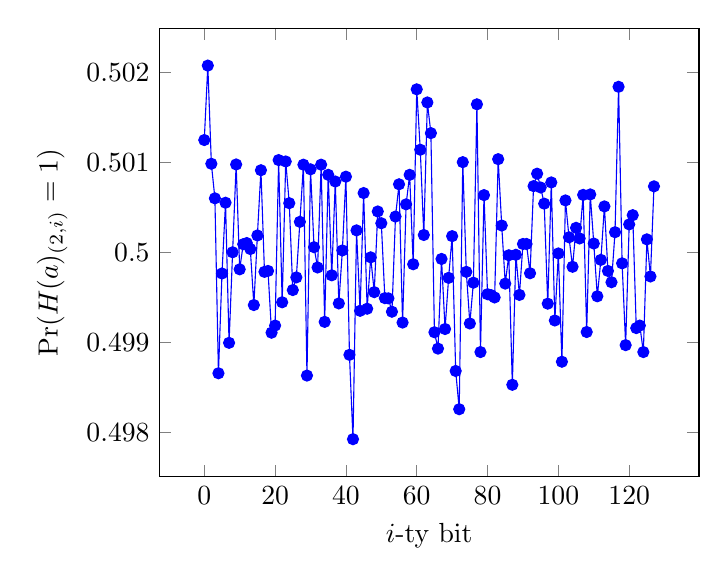
\begin{tikzpicture}
    \newcommand{\tmp}{$\Pr(H(a)_{(2,i)}=1)$}
    \begin{axis}[xlabel=$i$-ty bit,ylabel=\tmp,/pgf/number
    format/.cd,fixed,precision=3]
    \addplot[color=blue,mark=*] coordinates {
        (0, 0.501249577499)
        (1, 0.50207665441)
        (2, 0.500985834708)
        (3, 0.500601743263)
        (4, 0.498658240554)
        (5, 0.499766984524)
        (6, 0.50055309168)
        (7, 0.498996241025)
        (8, 0.50000256061)
        (9, 0.500978152879)
        (10, 0.499813075497)
        (11, 0.500092181947)
        (12, 0.500104984995)
        (13, 0.500038409144)
        (14, 0.499416181004)
        (15, 0.500189485113)
        (16, 0.500914137638)
        (17, 0.499784908791)
        (18, 0.49979515123)
        (19, 0.499108907849)
        (20, 0.499188286747)
        (21, 0.501026804462)
        (22, 0.49944690832)
        (23, 0.501011440804)
        (24, 0.500547970461)
        (25, 0.49958262063)
        (26, 0.49972345416)
        (27, 0.500340561081)
        (28, 0.500975592269)
        (29, 0.498632634458)
        (30, 0.500924380076)
        (31, 0.500058894021)
        (32, 0.499833560374)
        (33, 0.500975592269)
        (34, 0.499229256501)
        (35, 0.500862925445)
        (36, 0.499746499647)
        (37, 0.500788667766)
        (38, 0.499434105272)
        (39, 0.500023045487)
        (40, 0.500842440568)
        (41, 0.498863089324)
        (42, 0.4979259062)
        (43, 0.500245818524)
        (44, 0.499352165764)
        (45, 0.500660637285)
        (46, 0.49937521125)
        (47, 0.499946227198)
        (48, 0.499559575144)
        (49, 0.500455788514)
        (50, 0.500325197423)
        (51, 0.499492999293)
        (52, 0.499490438684)
        (53, 0.499341923325)
        (54, 0.500399455102)
        (55, 0.50075794045)
        (56, 0.499221574672)
        (57, 0.500535167413)
        (58, 0.500862925445)
        (59, 0.499869408909)
        (60, 0.501812911618)
        (61, 0.501142031895)
        (62, 0.500194606332)
        (63, 0.501666956869)
        (64, 0.501326395788)
        (65, 0.499114029068)
        (66, 0.498932225784)
        (67, 0.49992830293)
        (68, 0.499149877603)
        (69, 0.499718332941)
        (70, 0.500181803284)
        (71, 0.49868384665)
        (72, 0.498258785452)
        (73, 0.501003758975)
        (74, 0.499784908791)
        (75, 0.499211332234)
        (76, 0.499664560138)
        (77, 0.501646471992)
        (78, 0.49889381664)
        (79, 0.500637591798)
        (80, 0.499536529657)
        (81, 0.499526287218)
        (82, 0.499500681122)
        (83, 0.5010370469)
        (84, 0.500299591327)
        (85, 0.4996543177)
        (86, 0.499969272684)
        (87, 0.498530210072)
        (88, 0.499974393904)
        (89, 0.499528847828)
        (90, 0.500094742556)
        (91, 0.500094742556)
        (92, 0.499769545133)
        (93, 0.500737455573)
        (94, 0.500875728493)
        (95, 0.500722091916)
        (96, 0.500542849242)
        (97, 0.499431544662)
        (98, 0.500778425328)
        (99, 0.499244620159)
        (100, 0.499989757561)
        (101, 0.498786271035)
        (102, 0.500578697776)
        (103, 0.500169000236)
        (104, 0.499841242203)
        (105, 0.50027398523)
        (106, 0.500156197187)
        (107, 0.500640152407)
        (108, 0.499116589678)
        (109, 0.500645273627)
        (110, 0.500099863776)
        (111, 0.49951348417)
        (112, 0.499918060492)
        (113, 0.500512121926)
        (114, 0.49979515123)
        (115, 0.499669681358)
        (116, 0.500225333647)
        (117, 0.501841078324)
        (118, 0.499879651347)
        (119, 0.498970634929)
        (120, 0.500312394375)
        (121, 0.50041481876)
        (122, 0.499160120041)
        (123, 0.499188286747)
        (124, 0.49889381664)
        (125, 0.500145954749)
        (126, 0.499733696598)
        (127, 0.500734894964)
    };
    \end{axis}
\end{tikzpicture}
\caption{Przykładowy rozkład prawdopodobieństwa występowania "1" na kolejnych
bitach skrótów \texttt{MD5}, otrzymanych z zahaszowania 390532 wyrazów z
załącznika~\ref{att:english_wordlist}.}
\end{figure}
\pagebreak



\subsection{Zastosowania kryptograficznych funkcji skrótu}
\label{sec:secure_hash_usages}
Same funkcje skrótu mają bardzo szerokie zastosowania, my jednak skupimy się
wyłącznie na zastosowaniach \emph{kryptograficznych} funkcji haszujących. W
każdym przypadku opisane zastosowanie utylizuje podstawową cechę
kryptograficznych funkcji skrótu, jaką jest odporność na kolizje.

\subsubsection{Weryfikacja integralności danych}
\label{sec:usage_integrity_check}

Wyobraźmy sobie sytuację, w której użytkownik o imieniu Alicja zmuszony jest
przetransportować jakieś dane przez niebezpieczny kanał informacji, który jest
podatny na zakłócenia, do użytkownika imieniem Bob. Niech wiadomość wysłana
przez Alicję będzie $m$, a wiadomość odebrana przez Boba będzie $m'$.

\begin{figure}[htb!]
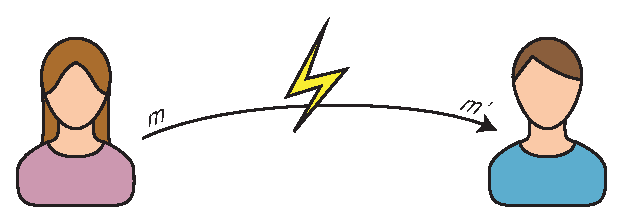
\includegraphics[width=10cm]{img/usage1.eps}
\caption{Wiadomość odebrana przez Boba niekoniecznie musi dotrzeć do niego w
formie identycznej jak podczas nadania przez Alicję}
\label{fig:usage_integrity_check_1}
\end{figure}

Z taką transmisją wiąże się wiele problemów, gdy zaczniemy rozpatrywać ją pod
kątem zapewnienia bezpieczeństwa. Jednym z takim problemów jest zapewnienie
bezpiecznego mechanizmu weryfikacji, czy dane odebrane przez Boba są faktycznie
tymi samymi danymi, które były wysłane do niego przez Alicję, a więc czy nie
zostały zmienione w jakikolwiek sposób podczas transportu. Innymi słowy, należy
w jakiś sposób zweryfikować, czy $m' = m$.

Z pomocą w rozwiązaniu tego problemu przychodzą funkcje haszujące. Alicja może,
obok samej wiadomości $m$, przesłać wyliczony u siebie skrót tej wiadomości,
$h=H(m)$. Bob może wówczas zweryfikować integralność odebranych danych $m'$
poprzez obliczenie ich skrótu po swojej stronie $H(m')=h'$, a w następnej
kolejności porównanie samych skrótów (sprawdzenie, czy obliczony przez Alicję
$h$ jest równy obliczonemu przez niego $h'$).

\begin{figure}[htb!]
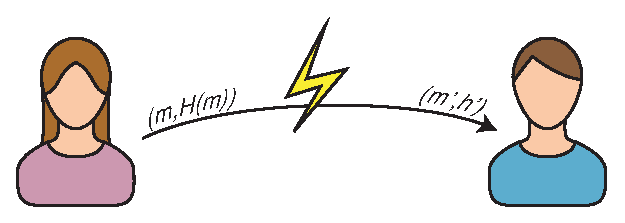
\includegraphics[width=10cm]{img/usage1b.eps}
\caption{Bob ma teraz dodatkowy mechanizm weryfikacji integralności --
wystarczy, że sprawdzi, czy $H(m')=h'$.}
\label{fig:usage_integrity_check_2}
\end{figure}

Wprowadzenie funkcji haszujących właśnie pozwoliło sprowadzić problem
zabezpieczenia transmisji potencjalnie bardzo długich komunikatów do
zabezpieczenia transmisji jedynie samych skrótów.

Należy zdawać sobie sprawę, że nie rozwiązuje to problemu zabezpieczenia
transmisji przed rozmyślnymi atakami -- jeśli ktoś mógł wcześniej edytować $m$,
teraz może również edytować wartość $h$ zawierającą $H(m)$. Ponadto funkcje
haszujące nie zapewniają żadnej poufności danych. Mimo to z ich zastosowania
płyną pewne wymienione niżej korzyści.

\begin{itemize}
\item Rozwiązanie to jest przydatne w sytuacjach, kiedy nie mamy do czynienia z
rozmyślnymi atakami, a jedynie przypadkowymi zakłóceniami --
prawdopodobieństwo, że skrót $H(m')$ będzie równy $H(m)$ w sytuacji, kiedy $m
\neq m'$ będzie minimalne. Jest to jedno z naturalnych zastosowań funkcji
haszujących, w których odgrywają rolę trudnej do podrobienia sumy kontrolnej.
\item Ponadto ułatwione jest napisanie innych protokołów -- dzięki funkcjom
haszującym zależy nam na zabezpieczeniu przed modyfikacją nie całej wiadomości,
a jedynie jej malutkiego kawałka zawierającego jej skrót. Przykładem protokołu,
który pracuje na opisanej powyżej zasadzie, jest podpis elektroniczny --
\emph{de facto} weryfikuje się tam wyłącznie autentyczność skrótu wiadomości, a
nie samą wiadomość.
\end{itemize}

\subsubsection{Bezpieczne przechowywanie / weryfikacja haseł}
\label{sec:usage_password_check}
Funkcje haszujące przychodzą z pomocą także w technikach przechowywania haseł.
Wyobraźmy sobie przeciętny mechanizm autentykacji...

\begin{enumerate}
\item Użytkownik Alicja przesyła swoje dane uwierzytelniające do serwera.
\item Serwer odbiera dane $m$.
\item Serwer porównuje dane $m$ z wzorcem $m'$ przechowywanym w bazie danych:
\label{enu:server_pass_check}
    \begin{enumerate}[label*=\arabic*.]
    \item jeżeli dane się zgadzają ($m = m'$), serwer udziela Alicji dostępu,
    \item w przeciwnym wypadku odmawia dostępu.
    \end{enumerate}
\end{enumerate}

Z takim podejściem wiąże się parę problemów. Po pierwsze, dane, która przesyła
Alicja, mogą zostać przechwycone przez osobę trzecią, zatem wymagają
zaszyfrowania (np. poprzez opakowanie transmisji protokołem \texttt{HTTPS}).
Jednak nie ten problem okazuje się ważny z punktu widzenia funkcji haszujących.
Nas zainteresuje problem wiążący się z punktem~\ref{enu:server_pass_check} --
co w wypadku, kiedy do bazy danych serwera, z jakichkolwiek przyczyn, uzyskuje
dostęp ktoś niepożądany? Taka osoba może wówczas podejrzeć dane
uwierzytelniające \emph{wszystkich} użytkowników, także Alicji, a następnie
pomyślnie zalogować przy pomocy tak wykradzionych danych.

Musimy zatem jakoś zabezpieczyć bazę danych. Można próbować ją szyfrować lub
inaczej zabezpieczać dane w niej przechowywane, problem z takim podejściem jest
jednak taki, że na pewnym poziomie tak czy inaczej jakaś osoba (administrator)
zawsze będzie miał dostęp do fizycznych danych. Możemy także zahaszować dane
uwierzytelniające i zmodyfikować nasz protokół w następujący sposób:

\begin{enumerate}
\item Użytkownik Alicja przesyła swoje dane uwierzytelniające do serwera.
\item Serwer odbiera dane $m$.
\item Serwer wylicza na ich podstawie hasz $h = H(m)$.
\item Serwer porównuje hasz $h$ z wzorcowym haszem $h'$ przechowywanym w bazie
danych:
    \begin{enumerate}[label*=\arabic*.]
    \item jeżeli skróty się zgadzają ($h = h'$), serwer udziela Alicji dostępu,
    \item w przeciwnym wypadku odmawia dostępu.
    \end{enumerate}
\end{enumerate}

Dzięki temu, że w bazie przechowywane są jedynie nieodwracalne skróty, nawet w
przypadku kradzieży bazy danych na podstawie wykradzionych skrótów nie powinno
być można odtworzyć oryginalnych danych (patrz
punkt~\ref{sec:preimage_resistance}). Teoretycznie zatem atakującemu taka baza
w zasadzie do niczego się nie przyda.

Należy jednak zwrócić uwagę, że protokół ten nie jest bezpieczny bez pewnych
poprawek. Przyczyny i natura poprawek omówione są w
części~\ref{sec:universal_attacks}.

\subsubsection{Jednoznaczna identyfikacja danych}

Innym zastosowaniem funkcji haszujących jest identyfikacja ciągów bajtów, a w
szerszym ujęciu -- plików, struktur/obiektów programistycznych itp. Poniżej
znajdują się przykłady wykorzystania tego pomysłu w różnego rodzaju
rozwiązaniach.
\begin{itemize}
\item Systemy kontroli wersji, w tym Mercurial oraz Git, wykorzystują funkcje
skrótu w celu bezpiecznej identyfikacji konkretnych wersji pliku, numerowania
kolejnych zmian i bezpiecznego przechowywania historycznej struktury
repozytorium.

\item Linki ed2k oraz magnet, używane w sieciach peer-to-peer, wykorzystują
funkcje skrótu w celu lokalizacji źródeł, skąd dany plik może być pobrany, a
także weryfikacji już ściągniętych danych (patrz
punkt~\ref{sec:usage_integrity_check}).
\item Struktury danych takie jak tablice mieszające (tzn. tablice, których
kluczami może być dowolny obiekt, w przeciwieństwie do klasycznych tablic o
indeksach liczbowych), wykorzystują funkcje haszujące do serializacji dowolnych
obiektów na taką postać, jaką ich algorytmy indeksowania są w stanie obsłużyć.
Przykładowo, w języku Java każdy zdefiniowany przez użytkownika obiekt powinien
zaimplementować metodę \texttt{hashCode()}, która w zamierzeniu ma pozwolić
łatwo odróżniać (na~tyle, na~ile to możliwe) konkretne instancje obiektu w
stosunku do pozostałych.
\end{itemize}

\begin{figure}[bht]
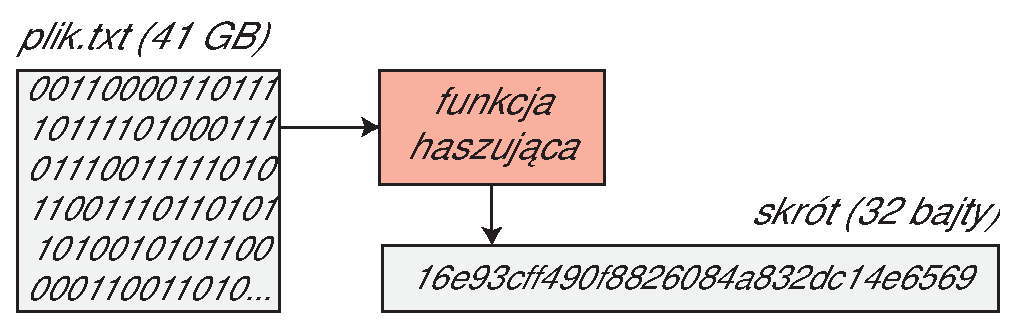
\includegraphics[width=12cm]{img/usage3.eps}
\caption{Gdy trzeba zweryfikować poprawność przesłania dużej struktury, łatwiej
porównać małą liczbę}
\end{figure}

Biorąc pod uwagę fakt, że kryptograficzne funkcje skrótu są dużo bardziej
kosztowne obliczeniowo niż zwykłe, nieodporne na ataki funkcje haszujące, w
większości tego typu zastosowań korzystanie z kryptograficznych funkcje skrótu
postrzegane jest jako przesada i stosowane są zwyczajne funkcje skrótu. Mimo
to, czasem jednak bezpieczeństwo jest konieczne, szczególnie w sytuacjach
opisanych powyżej, gdzie ryzyko ataku jest wysokie. Przykładowo, atakujący może
stworzyć plik zawierający wirus, którego hasz byłby taki sam jak skrót całkiem
niewinnego pliku, po czym umieścić taki plik w sieci peer-to-peer -- dzięki
zastosowaniu kryptograficznych funkcji skrótu, taki scenariusz jest bez
porównania trudniejszy do skutecznego przeprowadzenia.



\subsection{Rys historyczny}
Historia funkcji haszujących sięga późnych lat 70--tych. W roku 1976 Diffie i
Hellman w swojej pracy traktującej o kryptografii z kluczem publicznym, opisali
zapotrzebowanie na funkcję mapującą ciągi bitów dowolnej długości na ciągi
bitów ograniczonej długości w nieodwracalny sposób. W roku 1978 Rabin po raz
pierwszy zaproponował funkcję skrótu opartą na 64--bitowym wariancie blokowego
algorytmu szyfrującego DES. W 1979 roku Yuval opisał sposób, jak wykorzystując
paradoks urodzinowy złamać $n$--bitową funkcję haszującą w czasie $2^{n/2}$.

W tym samym roku zaczęły się pojawiać pierwsze próby zdefiniowania warunków,
jakie powinny spełniać bezpieczne funkcje skrótu. W 1979 Merkle wprowadził
pojęcie odporności na kolizje oraz odporności pierwszego i drugiego rzędu
(patrz sekcja~\ref{sec:secure_hash_attributes}). Definicje te zostały
ostatecznie sformalizowane przez Damg\r{a}rda w roku 1987. W roku 2004 Rogaway
i Shrimpton pokazali, że funkcje haszujące w miarę możliwości nie powinny być
odróżnialne od \textit{random oracles}.

Już od samego początku, czyli późnych lat 70--tych, funkcje haszujące
przeżywały bardzo szybki rozwój. Zapotrzebowanie na bezpieczne i szybkie
funkcje skrótu było szeroko rozumiane, nie zaskakuje zatem fakt, że do lat
90--tych znane było już około 50 konstrukcji. Pierwsi kandydaci korzystali z
dorobku blokowych funkcji szyfrujących; w późniejszym okresie rozwoju niektórzy
poszli w kierunku teoretycznych konstrukcji opartych na algebrze liniowej. Z
czasem jednak zaniechano adaptowania mechanizmów sprawdzonych w innych
zastosowaniach na rzecz tworzenia dedykowanych funkcji.

Tak naprawdę do dnia dzisiejszego niewiele się zmieniło: od lat
mamy do czynienia z ciągłym procesem wykazywania słabości istniejących
rozwiązań i w odpowiedzi wymyślania kolejnych usprawnień bądź całkiem nowych
konstrukcji. Proces ten zyskał nawet niedawno własne wydarzenie medialne w
postaci konkursu ogłoszonego przez National Institute of Standards and
Technology, mającego na celu wyłonienie następcy funkcji haszujących SHA-1 i
SHA-2 spośród kilkudziesięciu kandydatów zgłoszonych przez kryptologów z całego
świata. Cykl ten będzie prawdopodobnie trwał tak długo, aż zostanie odkryta
uniwersalna nieodwracalna funkcja skrótu lub wykazana zostanie niemożność
stworzenia takowej.



\section{Konstrukcja funkcji haszujących}
\label{sec:hash_construction}
Wprawdzie konstrukcji funkcji haszujących jest wiele, większość z nich wygląda
podobnie. Na początku skupię się na teoretycznych aspektach konstruowania
funkcji haszujących, a w następnej kolejności opiszę praktyczne implementacje.



\subsection{Doskonała funkcja skrótu}
W teorii mówi się o doskonałej funkcji skrótu, która każdy element $m$ z danego
zbioru $M$ potrafi przekształcić w sposób bezkolizyjny w $h$ z tego samego
zbioru. Innymi słowy, jest to bijekcja na samą siebie, lub permutacja.

\begin{figure}[htb!]
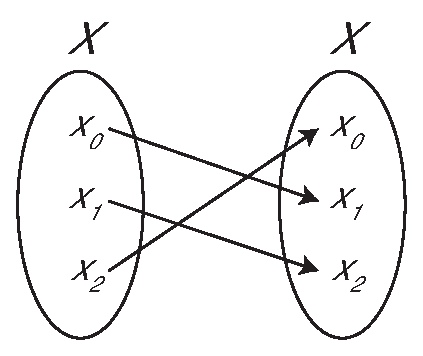
\includegraphics[width=6cm]{img/injection_self.eps}
\caption{Każdemu wyjściu przyporządkowywane jest dokładnie jedno wejście}
\label{fig:surjection}
\end{figure}


Znalezienie takiej funkcji w praktyce polega na użyciu algorytmu losowego,
który dobiera każdemu $m$ przypadkowy element $h$ tak długo, aż $h$ będzie
niewykorzystany przez żaden inny element (czyli zapewniony będzie brak
kolizji):

\begin{enumerate}
\item Zainicjuj tablicę podstawień $T$
\item Dla każdego $m \in M$:
    \begin{enumerate}[label*=\arabic*.]
        \item Wylosuj $h \in M$ takie, że $\not \exists_{m' \in M} : T_{m'} = h$
        \item Przydziel $T_m = h$
    \end{enumerate}
\end{enumerate}

Taka funkcja, mimo że na pierwszy rzut oka wydaje się przydatna w
zastosowaniach kryptograficznych (jak by nie patrzeć, implementuje całkowicie
losowe permutacje!), jest podejściem złym z prostych przyczyn:

\begin{itemize}
\item Algorytm przekształcania elementów $m \in M$ na $h$ polega na trywialnym
podstawianiu elementów zgodnie z jakąś tablicą $T$. Zatem, aby uzyskać
oryginalne $m$ na podstawie $h$ wystarczy odwrócić tablicę, zamieniając jej
klucze z przypisanymi im wartościami (dla danego $h$ wyszukać $m$, dla którego
$T_m = h$). Wykazaliśmy w ten sposób nieodporność na \textit{preimage
resistance}.
\item Gdy natomiast będziemy próbowali ukryć sposób w jaki dokonujemy
podstawienia (innymi słowy utajnić tablicę $T$), mamy do czynienia z
\textit{security through obscurity} (bezpieczeństwo poprzez niezrozumiałość),
co jest bardzo negatywnym zjawiskiem w kryptografii. System kryptograficzny
musi być bezpieczny nawet, gdy jego sposób działania wraz ze szczegółami
implementacji jest jawny (za wyjątkiem klucza, który jest z definicji tajny, z
tym że funkcje haszujące nie używają klucza).
\item Nawet gdy zignorujemy powyższe przykazanie, nasz algorytm będzie
nieodporny na proste ataki statystyczne: analizując rozkład prawdopodobieństwa
pewnych wzorców wewnątrz kolejnych $h$ (który nie jest jednostajny, jako że w
praktyce rzadko kiedy wejście ma rozkład jednostajny), możemy zyskać ogólne
wyobrażenie o tym, jak wyglądają wzorce wewnątrz $m \in M$, co może nas
doprowadzić do oryginalnych $m$.
\item Wreszcie, funkcja taka jest bardzo niepraktyczna: po pierwsze, musimy
znać z góry \emph{wszystkie} możliwe wiadomości, jakie możemy chcieć
zahaszować; mało tego -- wiadomości te muszą mieć tę samą długość. Powoduje to,
że funkcja ta nie nadaje się na kryptograficzną funkcję skrótu.
\end{itemize}



\subsection{Funkcja jednokierunkowa}
Funkcja jednokierunkowa to funkcja, której wartości dla każdego wejścia da się
łatwo obliczyć; powinno być trudne natomiast obliczenie wejścia na podstawie
posiadanego konkretnego wyjścia.

\noindent
Nieformalnie, funkcja $f$ jest silnie jednokierunkowa, jeśli:
\begin{itemize}
\item da się obliczyć w czasie wielomianowym (czyli w taki sposób, że czas
działania $f$ jest w sposób wielomianowy zależny od rozmiaru danych
wejściowych),
\item żaden probabilistyczny algorytm działający w czasie wielomianowym nie
potrafi zgadnąć argumentu z zaniedbywalnie małym prawdopodobieństwem.
\end{itemize}

\noindent
$f$ jest natomiast słabo jednokierunkowa, jeśli:
\begin{itemize}
\item da się obliczyć w czasie wielomianowym,
\item każdy probabilistyczny algorytm działający w czasie wielomianowym zgaduje
argumenty w sposób poprawny z zaniedbywalnie małym prawdopodobieństwem.
\end{itemize}

Łatwo zauważyć, że każda silnie jednokierunkowa funkcja spełnia jednocześnie
warunki nałożone na funkcje słabo jednokierunkowe. Ponadto każda funkcja
jednokierunkowa spełnia automatycznie podstawowy warunek nałożony na bezpieczne
funkcje skrótu (mianowicie \textit{preimage collision resistance}). Funkcje te
powinny zatem przyciągnąć nasze zainteresowanie.

\subsubsection{$\textrm{P} \neq \textrm{NP}$?}
Problem z funkcjami jednokierunkowymi jest niestety taki, że... nie udowodniono
ich istnienia. Istnieją pewne funkcje, które podejrzewamy o jednokierunkowość,
lecz nie potrafimy wykazać poprawności lub niepoprawności tego podejrzenia.
Wykazano, że z istnienia słabo jednokierunkowych funkcji wynika istnienie
silnie jednokierunkowych funkcji. Ponadto udowodniono, że istnienie funkcji
jednokierunkowych implikowałoby jednocześnie, że $\textrm{P} \neq \textrm{NP}$,
co dałoby odpowiedź na jeden z problemów milenijnych i oznaczałoby, że klasa
problemów, które da się \emph{rozwiązać} w czasie wielomianowym ($\textrm{P}$)
nie pokrywa się z klasą, dla którego rozwiązanie da się \emph{zweryfikować} w
czasie wielomianowym ($\textrm{NP}$). Przykładowo: mając liczbę $x \in
\mathbb{N}$ i dany zbiór liczb pierwszych $x_i$, możemy w banalny sposób
\emph{zweryfikować}, czy $x_0 \cdot x_1 \cdot \ldots \cdot x_n = x$. Natomiast
nie wiadomo, czy istnieje algorytm wielomianowy, który potrafi \emph{rozwiązać}
ten problem, znajdując dla danego $x$ liczby pierwsze $x_0, x_1, \ldots, x_n$
takie, że $x_0 \cdot x_1 \cdot \ldots \cdot x_n = x$. Problem ten jest znany
jako problem rozkładu liczby na czynniki pierwsze, lub inaczej problem
faktoryzacji, i stanowi pierwszy ze wspominanych kandydatów na funkcje
jednokierunkowe.

\subsubsection{Problem faktoryzacji}
Niech $f(S) = \prod_{s \in S} s$, gdzie $S$ jest dowolnym zbiorem liczb
pierwszych oraz $x \in \mathbb{N}$. Obliczenie $f(S)$ jest trywialne. Natomiast
obliczenie wartości odwróconej funkcji $f^{-1}(x)=S$, a więc znalezienie dla
danej liczby $x$ jej czynników pierwszych, jest trudne, tzn. nieznany jest
żaden algorytm, który by to potrafił realizować w czasie zależnym wielomianowo
od rozmiaru $x$.

\subsubsection{Problem logarytmu dyskretnego}
Niech $f(x, p, g) = g^x \mod p$, gdzie $p$ jest liczbą pierwszą, $g < p$ oraz
$x < p$. Wyliczenie tej wartości jest trywialne; nie znamy natomiast algorytmu
wielomianowego pozwalającego na zgadnięcie wartości odwróconej funkcji
\mbox{$f^{-1}(y, p, g) = x : g^x \mod p = y$} na podstawie danego $y$. Nazwa problemu
wynika z charakteru $f$ (operacją odwrotną do potęgowania w ciele modulo $p$
jest logarytm w ciele modulo $p$).

\subsubsection{Funkcja Rabina}
Niech $f(x,n) = x^2 \mod n$. Wykazano, że obliczenie $f^{-1}(y,n) = x : x^2
\mod n = y$ na podstawie $y$ i $n$ jest tak samo trudne, jak rozkład $n$ na
czynniki pierwsze; co sprowadza się do problemu faktoryzacji, opisanego
wcześniej.

\subsubsection{Wnioski}
Zastosowania funkcji jednokierunkowych są niejako podzbiorem tego, do czego
potrzebujemy bezpiecznych funkcji haszujących: łatwe obliczenie $f(x)$, łatwa
weryfikacja $f(x)=f(x')$ i trudne uzyskanie odwróconej funkcji $f^{-1}(y)=x$.
Stąd też nie powinno dziwić, że ostatnim, niewspomnianym dotąd kandydatem na
funkcje jednokierunkowe są... kryptograficzne funkcje skrótu.

Zapotrzebowanie na funkcje jednokierunkowe jest duże, o czym świadczy ich
wykorzystanie: trudność faktoryzacji jest zastosowana w kryptosystemie RSA,
trudność obliczenia logarytmu dyskretnego w podpisach cyfrowych ElGamala, a
trudność obliczenia pierwiastka dyskretnego (funkcja Rabina) - w kryptosystemie
Rabina. Trudność złamania tych kryptosystemów opiera się właśnie na trudności
odwrócenia wymienionych funkcji.

Wracając na chwilę do zagadnienia $\textrm{P} \stackrel{?}{=} \textrm{NP}$ --
wystarczy udowodnić, że którakolwiek z powyższych funkcji jest faktycznie
jednokierunkowa lub pokazać, że może zostać złamana, by móc stwierdzić to samo
o wszystkich pozostałych wymienionych funkcjach. Jest tak dlatego, ponieważ
istnieją sposoby przekształcania jednego problemu w drugi tak, że rozwiązanie
jednego gwarantuje rozwiązanie drugiego. Zatem tak naprawdę bezpieczeństwo
powyższych kryptosystemów jest do pewnego stopnia ekwiwalentne (na tyle, na ile
kosztowne są przekształcenia problemów).



\subsection{Formalnie bezpieczne funkcje skrótu}
Implementacje funkcji skrótu dzielą się na dwie kategorie. Pierwsza z nich,
omówiona tutaj, wywodzi się z formalnego spojrzenia na problem haszowania. Tak
naprawdę metoda ta sprowadza się do wykorzystania opisanych wcześniej
kandydatów na funkcje jednokierunkowe i dostarczeniu dowodu, że złamanie
konstrukcji opartej na danym problemie jest tak samo trudne, jak trudne jest
rozwiązanie tego problemu. Z charakteru tego podejścia wywodzi się nazwa tej
rodziny kryptograficznych funkcji haszujących: \textit{provably secure
cryptographic hash functions}.

W praktyce dowody trudności złamania funkcji z tej rodziny polegają na
pokazaniu istnienia algorytmu, który przekształca w czasie wielomianowym
problem znajdowania kolizji dla takiej funkcji w problem rozwiązania źródłowego
problemu. W ten sposób, kiedy zostanie znaleziony algorytm wielomianowy
potrafiący złamać formalną funkcję haszującą, będzie od razu znany sposób
szybkiego rozwiązywania problemu leżącego pod tą funkcją -- a na chwilę obecną
zakłada się, że problemy te (faktoryzacja, znajdywanie logarytmu dyskretnego
itp.) są nierozwiązywalne w czasie wielomianowym, tak więc oznacza to
(najprawdopodobniej) sprzeczność. Możemy zatem powiedzieć, że trudność złamania
formalnych funkcji skrótu jest nie mniejsza niż trudność rozwiązania dowolnego
problemu, o którym podejrzewamy, że jest trudny do rozwiązania. Innymi słowy,
problem złamania takich funkcji jest redukowalny do problemu milenijnego, stąd
funkcje te są postrzegane jako najbezpieczniejsze dostępne warianty.



\subsection{Współczesne implementacje}
Wprawdzie formalnie bezpieczne funkcje skrótu są bardzo bezpieczne, nie
przychodzi to bez kosztów. Praktyka pokazuje, że funkcje te prawie w ogóle się
nie nadają do zastosowań praktycznych lub przemysłowych z racji swojego wolnego
działania lub wysokich kosztów pamięciowych; niestety, skutecznie eliminuje to
ich przydatność wszędzie tam, gdzie mamy do czynienia z ograniczonymi zasobami
(przykładami mogą być: systemy wbudowane, transmisje danych w czasie
rzeczywistym czy też systemy uwierzytelniania o dużej przepustowości).

W związku z tym została stworzona druga rodzina kryptograficznych funkcji
skrótu. Działanie funkcji z tej rodziny polega ogólnie rzecz biorąc na
dokonywaniu ogromnych ilości różnorodnych operacji na konkretnych bitach
wiadomości $m$ (takich, jak przestawianie, dodawanie, odejmowanie i inne).
Komputery są przystosowane do tego typu obliczeń, dzięki czemu w porównaniu do
formalnie bezpiecznych funkcji skrótu haszowanie takimi funkcjami odbywa się
bardzo szybko. Oznacza to jednak, że autorzy funkcji zazwyczaj ograniczają się
jedynie do wstępnej analizy jej słabości, \textit{de facto} nie przedstawiając
formalnego dowodu trudności jej złamania. Badania mające na celu znalezienie
słabości przypominają w swojej naturze szukanie igły w stogu siana:
nieznalezienie igły na daną chwilę nie oznacza jeszcze nieistnienia igły. Daje
to pole do popisu kryptologom, którzy znajdują luki na długo po tym, jak dana
funkcja została opisana po raz pierwszy.

\subsubsection{Konstrukcja Merkle-Damg\r{a}rda}

\subsubsection{MD5}

\subsubsection{SHA-1}

\section{Ataki uniwersalne}
\label{sec:universal_attacks}

\subsection{Atak brutalny}

\subsection{Atak słownikowy}

\subsubsection{Odwrócony atak słownikowy}

\subsection{Tęczowe tablice}

\subsection{Ataki typu Denial of Service}

\section{Ataki teoretyczne}

\subsection{Ataki na słabe funkcje haszujące}

\subsubsection{\textit{Collision resistance}}

\subsubsection{\textit{Preimage resistance}}

\subsubsection{\textit{Second preimage resistance}}

\section{Podsumowanie}

\section{Bibliografia}

\section{Załączniki}

\begin{enumerate}
\item \refstepcounter{attcounter}\label{att:english_wordlist}Lista
przypadkowych, niepowtarzających się angielskich wyrazów używana do
przeprowadzania testów statystycznych.
\url{http://download.openwall.net/pub/wordlists/languages/English/3-large/lower.gz}
\end{enumerate}

\end{document}
